\scanpage{541}
\mspage{276}

\unsure{(12)} where $\Sigma$ \inserted{$\subset\mathbb C$} is \unsure{the subextension} that is maximal cyclotomic in $\overline{\mathbb Q}_0$.

\deleted{\unsure{The}} We recover the $M_{1,1}[n']$, for $n'\mid n$, \inserted{$n'\ne 1,2$,} from $M_{1,1}[n]$ with the action of $\Gamma_n$ on it, by
\[
(13)\qquad M_{1,1}[n']\simeq M_{1,1}[n]\wedge_{\Gamma_n}\Gamma_{n'}\simeq M_{1,1}[n]/K_{n,n'}
\]
\[
\text{over }\operatorname{Spec}\mathbb Z[1/n]
\]
where
\[
(14)\qquad K_{nn'}=\operatorname{Ker}(\Gamma_n\longrightarrow\Gamma_{n'}).
\]

\margin{\uline{N.B.} $K_{n,n'}$ operates \uline{freely} on the scheme $M_{1,1}[n]$ (if $n'\mid n$, $n'\ne 1,2$) --- but of course not if $n'=1$ or $2$.}

If however we apply this formula in \unsure{the inadmissible case|the inadmissible cases} $n'=1$ or $2$, we find for the case $n'=1$, not $M_{1,1}$ but $\widetilde M_{1,1}$ (coarse modular scheme), and for $n'=2$, not $M_{1,1}[2]$ (which is not a scheme either) but what we had called in the preceding \S\ $M_{1,1}[2]'$.

We can \deleted{\unsure{determine|define}} \inserted{make explicit} \inserted{$M_{1,1}$ and} $\widetilde M_{1,1}$ over all of $\operatorname{Spec}\mathbb Z$, \inserted{in terms of the $M_{1,1}[n]$,} by describing them \inserted{over the} two open sets $\operatorname{Spec}(\mathbb Z[1/n])$, $\operatorname{Spec}(\mathbb Z[1/n'])$ which cover $\operatorname{Spec}(\mathbb Z)$ (i.e. for $(n,n')=1$) by (9) and (10), \inserted{(taking first $n$, then $n'$ in them)} and by ``gluing'' \deleted{in} over $\operatorname{Spec}(\mathbb Z[\frac{1}{nn'}])$ by these same formulas, applied to $nn'$\ldots

\scanpage{542}

We have moreover (for the record)
\[
\text{\uline{Theorem}}\qquad \widetilde M_{1,1}\simeq\mathbb E^1_{\mathbb Z}\qquad(\text{over }\operatorname{Spec}\mathbb Z)
\]

We can pin down such an isomorphism (\unsure{defined|defines} a priori modulo the integral affine group $X\longmapsto\pm X+n$, $n\in\mathbb Z$) by \unsure{noting} that there are in $\widetilde M_{1,1}$ two distinguished sections over $\mathbb Z$, whose values at the generic point correspond to the two isomorphism classes of elliptic curves in characteristic $0$ (over $\mathbb C$, for example) which have automorphisms $\ne\mathrm{id},-\mathrm{id}$ --- the two groups \unsure{of automorphisms} that we obtain are moreover $\mathbb Z/4\mathbb Z$ and $\mathbb Z/6\mathbb Z$ (very easy for example by the \unsure{transcendental|transcendental} route). These are what are called unless I am mistaken the ``anharmonic'' elliptic curves. On an $M_{1,1}[n]$, the group of rational automorphisms\,$/k$ of an elliptic curve described by a point $x$ of $M_{1,1}[n](k)$ is canonically identified with the stabilizer of $x$ in $\Gamma_n$:
\[
(15)\qquad\operatorname{Aut}(E_x)\simeq(\Gamma_n)_x
\]

\scanpage{543}
\mspage{277}

--- of course, we have suitable statements over an arbitrary base scheme, not necessarily a field. This already shows that the \unsure{automorphisms} of elliptic curves are linked in an essential way to the \uline{ramification} of $\Gamma_n$ operating on $\unsure{M_{1,1}[n]|M_{1,n}[n]}$. We thus find:

\uline{Proposition} (Over $\operatorname{Spec}\mathbb Q$) There are exactly two orbits of $\Gamma_n$ operating on $M_{1,1}[n]$ which are ``\deleted{singular}\inserted{critical}'', and which correspond to stabilizers isomorphic resp. to $\mathbb Z/4\mathbb Z$ and $\mathbb Z/6\mathbb Z$, which are the groups of \unsure{automorphisms} of the corresponding (``anharmonic'') elliptic curves.

\margin{$n\ne 1,2$}

We \unsure{will note|note} that $\Gamma_n$ \uline{does not operate} \unsure{faithfully|faithfully} on $M_{1,1}[n]$ --- the kernel of this operation is the central subgroup $\{\pm1\}$, image of the corresponding group of $\operatorname{Gl}(2,\mathbb Z)$ --- it corresponds to the group of ``universal'' automorphisms $\pm\mathrm{id}_E$ of elliptic curves $E$. The quotient group
\[
(16)\qquad \Gamma'_n=\Gamma_n/\{\pm1\}
\]
\deleted{\unsure{(on|on}} operates \unsure{faithfully|faithfully}, and we can look at the ``mixed topos'' $(M_{1,1}[n],\Gamma'_n)$ --- we find

\scanpage{544}
at once that it \uline{does not depend} (up to canonical \unsure{equivalence|equivalence}) \uline{on the choice of} $n$ [except that the open set of $\operatorname{Spec}\mathbb Z$ over which ``it makes sense'' depends on $n$\dots] -- and. in fact, we have:

\margin{thus on \unsure{condition} of working over a base scheme (such as $\operatorname{Spec}\mathbb Z[\frac{1}{nn'}]$) where $n,n'$ are \unsure{both} invertible\dots}

\[
(17)\qquad (M_{1,1}[n],\Gamma'_n)\simeq M_{1,1}'
\]
\[
(\text{over }\operatorname{Spec}\mathbb Z[1/n])
\]
where the modular \deleted{topos} \inserted{schematic multiplicity} $M_{1,1}'$ is \unsure{described|described}, in terms of elliptic curves ``\unsure{defined} modulo symmetry'', as in the \S\ preceding.

\uline{Remark.} The preceding proposition seems to depend on $n$ -- but we see a priori \deleted{that} (thanks to the fact that the $\Gamma_{n,n'}$ \inserted{($n'\mid n$, $n'\ne1,2$)} (\unsure{operating|operate} freely) that if it is valid for \uline{one} $n$, it is valid for all.

\deleted{\unsure{Corollary}} Let us note \deleted{that} also

\uline{Corollary of the proposition.} \inserted{(characteristic 0)} The stabilizers \uline{in $\Gamma'_n$} (the group which operates \uline{\unsure{faithfully}} on $M_{1,1}[n]$) of the points of the \unsure{two} critical orbits are resp. $\mathbb Z/2\mathbb Z$ and $\mathbb Z/3\mathbb Z$. \deleted{\illegible{1}}

\margin{valid for $n\unsure{\ne|=|\geq}2$, \unsure{cf.|cf.} below}

\scanpage{545}
\mspage{278}
We have assumed here that $n\ne1,2$ -- but nothing prevents us from also considering \inserted{on}
\[
(18)\qquad M_{1,1}[2]'\overset{\mathrm{dfn}}{=}M_{1,1}[2m]/\Gamma_{2m,2}
=M_{1,1}[2m]/\unsure{\Gamma_{2m,2}|\Gamma'_{2m,2}}
\]
(where $m$ is any integer, $\ge2$)
the action of $\Gamma_2\simeq\operatorname{Gl}(2,\mathbb Z/2\mathbb Z)\simeq\operatorname{Sl}(2,\mathbb Z/2\mathbb Z)\simeq\unsure{\mathfrak S_3|\mathcal S_3}\simeq\Gamma_{2m}/\Gamma_{2m,2}$. \deleted{\unsure{Whereas|Whereas}} It is no longer true, \inserted{to be sure,} that $\Gamma_{2m,2}$ operates \unsure{freely} on $M_{1,1}[2m]$ -- for $\Gamma_{2m,2}$ contains the element $-1\in\Gamma_{2m}$ corresponding to the universal symmetry $-\operatorname{id}_E$ -- i.e. \inserted{\unsure{to}} the element \deleted{\unsure{of}} $-1$ of $\operatorname{Gl}(2,\mathbb Z)$. But the general rigidity result recalled at the beginning implies that \deleted{$\Gamma'_{2m,2}=\Gamma_{2m,2}/\pm1$}
\[
(19)\qquad\Gamma'_{2m,2}\overset{\mathrm{dfn}}{=}\Gamma_{2m,2}'/\pm1
\simeq\operatorname{Ker}(\Gamma'_{2m}\longrightarrow\Gamma'_2\simeq\unsure{\mathfrak S_3|\mathcal S_3})
\]
operates \deleted{\unsure{fi}} \inserted{still} \uline{freely} on $M_{1,1}[2m]$ -- and this implies that the corollary of the proposition is still valid for the action of $\Gamma'_2\,(\xleftarrow{\sim}\Gamma_2\simeq\unsure{\mathfrak S_3|\mathcal S_3})$ on $M_{1,1}[2]'$.

\uline{Terminological digression.} $M_{1,1}$ \inserted{${}=M_{1,1}[1]$} and the

\scanpage{546}
\mspage{278}
\figure{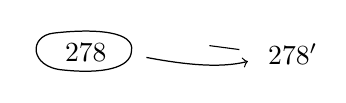
\begin{tikzpicture}[x=1cm,y=1cm,baseline=(ancien.base)]
\node[inner sep=0pt] (ancien) at (0,0) {$278$};
\draw[line width=0.45pt]
  (0.58,0.02) .. controls (0.63,0.27) and (0.13,0.31) .. (-0.40,0.25)
  .. controls (-0.73,0.22) and (-0.72,-0.19) .. (-0.28,-0.22)
  .. controls (0.20,-0.27) and (0.57,-0.20) .. (0.58,0.02);
\draw[->,line width=0.45pt]
  (0.77,-0.06) .. controls (1.25,-0.15) and (1.70,-0.20) .. (2.06,-0.11);
\draw[line width=0.4pt] (1.57,0.09) -- (1.95,0.04);
\node[anchor=west,inner sep=0pt] at (2.31,-0.015) {$278'$};
\end{tikzpicture}}
\mspage{278'}
$M_{1,1}[n]$ ($n\in\mathbb N^*$) are \unsure{defined} \unsure{a|a} priori as modular schematic \uline{multiplicities}, i.e. a) as locally ringed topoi locally isomorphic to the étale topos of a scheme (in this case, of finite type over $\operatorname{Spec}\mathbb Z$, or over $\mathbb Q$ if we work in characteristic 0) and b) \unsure{defined}, up to equivalence itself defined up to unique \unsure{isomorphism|isomorphism}, as ``representing'' the \deleted{\illegible{1}} corresponding ``functors''
\[
S\longmapsto
\begin{gathered}
\text{category of elliptic curves}\\
\text{relative over }S\text{, with rigidification}\\
\text{of Jacobi of level }n\text{ i.e.}\\
\text{isomorphism}\quad(\mathbb Z/n\mathbb Z)_S\simeq{}_nE\\
={}\unsure{\mathcal{E}ll_n}(S)
\end{gathered}
\]
thus by construction we have \inserted{for every scheme $S$} an equivalence
\[
\unsure{\mathcal{E}ll_n}(S)\unsure{\simeq|\cong}
\text{\uline{$\operatorname{Hom}$}}_{\substack{\text{topoi locally}\\\text{ringed}\\\text{i.e. morphisms of}\\\text{multiplicities}}}
(S,M_{1,1}[n])
\]
For the categories $\unsure{\mathcal{E}ll_n}(S)$ to be \uline{discrete}, \deleted{\illegible{1}} or again for $M_{1,1}[n]$ to be a scheme, or again for the automorphisms of an

\scanpage{547}
\mspage{279}

elliptic curve \unsure{respecting|respect} a Jacobi rigidification of level $n$ \unsure{to be} the identity, it \unsure{is necessary and sufficient} that $n\geq 3$ i.e. $n\neq 1,2$. Thus $M_{1,1}[2]$ \uline{is not} a scheme -- but $M'_{1,1}[2]$ is one, and $M_{1,1}[2]\to M_{1,1}[2]'$ is a \deleted{\illegible{1}} local isomorphism (described entirely by a $\mathbb Z/2\mathbb Z$-gerbe over $M_{1,1}[2]'$). \deleted{\unsure{We consider of course}} \inserted{\unsure{It} is necessary all the same to take the} trouble to define
\diagram{\[
\tag{20}
\begin{tikzcd}[ampersand replacement=\&,column sep=large,row sep=large]
M_{1,1}[2] \arrow[r] \arrow[d,phantom,"{\simeq}"{description,rotate=90},"{\text{``theorem''}}"{description,xshift=3em}] \& M_{1,1}[2]' \arrow[d,phantom,"{\simeq}"{description,rotate=90},"{\text{``definition''}}"{description,xshift=3em}] \\
(M_{1,1}[2m],\Gamma_{2m,2}) \& M_{1,1}[2m]/\Gamma'_{2m,2} \arrow[d,phantom,"{\Vert}"{description}] \\
\& M_{1,1}\unsure{(2m)|[2m]}/\Gamma_{2m,2}
\end{tikzcd}
\]}
as the canonical homomorphism of ``passage to the coarse quotient'' -- which makes sense whenever a discrete group (say)\unsure{\S} $G$ operates on a scheme (say) $X$, as a morphism
\[
\tag{21}
(X,G)\longrightarrow X/G=Y
\]
whose inverse \unsure{image} functor (sheaves on $Y=X/G\longrightarrow G$-sheaves on $X$) is obvious. Here we have a normal subgroup \unsure{$\mathfrak z$|$z$} of $G$ which operates \unsure{trivially|trivially} on $X$, such that $G/\unsure{\mathfrak z|z}$ operates freely, which means that the morphism

\scanpage{548}

(21) factors as
\[
\tag{22}
(X,G)\longrightarrow
\left(X,\underbrace{G/\unsure{\mathfrak z|z}}_{G'}\right)
\overset{\sim}{\longrightarrow}Y=X/G=X/G',
\]
so that the morphism of multiplicities (21) is also identified, simply, with
\diagram{\[
\tag{23}
\begin{tikzcd}[ampersand replacement=\&,column sep=large,row sep=large]
(M_{1,1}[2m],\Gamma_{2m,2}) \arrow[r] \& (M_{1,1}[2m],\Gamma'_{2m,2}) \arrow[d,phantom,"{\simeq}"{description,rotate=90}] \\
\& M_{1,1}[2]'
\end{tikzcd}
\]}

On the other hand, if we want to go down as far as $M_{1,1}[1]'=M_{1,1}'$, by passing to the quotient (in the ``coarse'' sense) of $M_{1,1}[n]$ by $\Gamma'_n$, the morphism
\diagram{\[
\tag{24}
\begin{tikzcd}[ampersand replacement=\&,column sep=large,row sep=large]
(M_{1,1}[n],\Gamma'_n) \arrow[r] \arrow[d,phantom,"{\Vert}"{description}] \& M_{1,1}[n]/\Gamma'_n \arrow[d,phantom,"{\Vert}"{description}] \\
M_{1,1}' \& \widetilde M_{1,1}
\end{tikzcd}
\]}
is no longer an ``isomorphism'' i.e. is no longer an equivalence, for $\Gamma'_n$ does not operate freely -- it has \inserted{(even in characteristic $0$)} ramification of degree $2,3$.

[If however we exclude the anharmonic elliptic curves, \unsure{its|it} would work -- it is ``only in the neighborhood'' of these elliptic curves that (24) is not an isomorphism\ldots

\scanpage{549}
\mspage{280}

In fact, the arguments of the preceding \S{} establish an isomorphism (\unsure{valid} over \inserted{the} $\mathrm{Spec}\,\unsure{\mathbb Z[1/n]}$ of $\mathbb Z[1/2]$)
\[
(25)\qquad M_{1,1}[2]'\simeq M_{0,4}^{!}\simeq U_{0,3}
\]
(\unsure{valid} over $\mathrm{Spec}\,\mathbb Z[1/2]$)

\margin{N.B. \unsure{the image} of $M_{1,1}[2]'$ in $\mathrm{Spec}\,\mathbb Z$ is $\mathrm{Spec}\,\mathbb Z[1/\unsure{n|2}]$, while that of $M_{0,4}^{!}\simeq U_{0,3}$ is $\mathrm{Spec}\,\mathbb Z$ in \unsure{all} its entirety}

and this isomorphism is compatible with the operations of \deleted{$\unsure{\Gamma'_2\simeq\Gamma}$}
\[
(26)\qquad \Gamma'_2\simeq\Gamma_2=\operatorname{Gl}(2,\mathbb Z/2\mathbb Z)=\operatorname{Sl}(2,\mathbb Z/2\mathbb Z)
\]
on $M_{1,1}[2]'$ on the one hand, of $\unsure{\mathfrak S_3|\mathcal S_3}$ on $U_{0,3}$ on the other \unsure{hand|hands}, when we consider the isomorphism
\[
(27)\qquad
\begin{array}{ccc}
\Gamma_2 & \xrightarrow{\sim} & \unsure{\mathfrak S_3|\mathcal S_3}\\
\Vert &&\\[-4pt]
\operatorname{Gl}(2,\mathbb F_2)&&
\end{array}
\]
which associates, to every automorphism of $\mathbb F_2^2$, its action on the three nonzero elements, $\underline{\alpha}=(1,0)$, \inserted{$\underline{\beta}=$}$(0,1)$, and $\underline{\gamma}=(1,1)=\underline{\alpha}+\underline{\beta}$ (so that we have moreover) \deleted{\illegible{2}}
\[
(28)\qquad \gamma=\alpha\unsure{+|-}\beta,\quad \unsure{\alpha|\beta}=\beta\unsure{+|-}\gamma,\quad \beta=\unsure{\gamma}+\alpha.
\]
It would be necessary to make this compatibility explicit, by \unsure{considering} the natural action of $\unsure{\mathfrak S_4|\mathcal S_4}$ on $M_{0,4}^{!}$, $M_{0,n}^{!}$ being the modular multiplicity defined by

\scanpage{550}

\[
(29)\qquad
\underline{\operatorname{Hom}}_{\text{multiplicities}}(S,M_{0,n}^{!})\simeq
\begin{gathered}
\text{category of}\\
\text{relative \unsure{curves|lines}}\\
\text{over }S,\ \text{locally isomorphic to }\mathbb P^1_S\\
\text{(for étale topology) and equipped}\\
\text{with }n\text{ sections mutually}\\
\text{\unsure{disjoint} \unsure{numbered}}\\
\deleted{\illegible{1}}\quad\unsure{s_1|s_0},s_2,\ldots s_n
\end{gathered}
\]

\margin{If we want representability for $n=0,1,2$, it no longer suffices to work with \unsure{the étale topology|the étale topologies} --- we need fppf topologies for example...}

\uline{N.B.} this really is representable by a multiplicity iff $n\geq3$, \inserted{i.e. if the stack \unsure{in|of} groupoids which we want to \unsure{represent} is ``rigid'' ---} and then the multiplicity is even a scheme, isomorphic moreover \unsure{canonical|canonically} to the \inserted{\unsure{sub-}}scheme
\[
\underline{\operatorname{Mon}}(I_{n-3},U_{0,3})\subset U_{0,3}^{I_{n-3}},
\]
where here
\[
I_{n-3}=\{i\in\mathbb N\quad3<i\leq n\deleted{\unsure{-3}}\}
\]
--- thus \deleted{\illegible{1}}
\[
M_{0,3}^{!}\xrightarrow{\sim}\mathrm{Spec}\,\mathbb Z\quad\text{(terminal scheme)},\quad\text{and}
\]
\[
M_{0,4}^{!}\xrightarrow{\sim}U_{0,3}=\mathbb P^1_{\mathbb Z}\setminus\{\text{sections \deleted{\illegible{1}} }0,1,\infty\}=\mathrm{Spec}\,\mathbb Z[T]\Bigl[\frac{1}{T(T-1)}
\]

But we will keep in mind that there is a natural operation of $\unsure{\mathfrak S_n|\mathcal S_n}$ on $M_{0,n}^{!}$, hence on $\underline{\operatorname{Mon}}(I_{n-3},U_{0,3})$ --- \deleted{\unsure{of which|therefore}} whereas we see a priori only the action of $\unsure{\mathfrak S_3|\mathcal S_3}\times\unsure{\mathfrak S_{n-3}|\mathcal S_{n-3}}$ on the latter: the canonical isomorphism
\[
(30)\qquad M_{0,n}^{!}\simeq\unsure{\operatorname{Mon}}(I_{n-3},U_{0,3})\subset U_{0,3}^{I_{n-3}}
\]
\[
\text{(where }I_{n-3}=\{i\in\mathbb N\mid\deleted{\unsure{2}}3<i\leq n\}\text{)}
\]
takes account only of the natural operations \unsure{of the|of the}